\documentclass[a5paper, 10pt]{tekst}

\usepackage{titlesec}



\begin{document}
	\thispagestyle{empty}
	\onehalfspacing
	\titleformat*{\section}{\sffamily\bfseries}
	\sffamily
	
	\begin{center}
		\Huge 地震が起こったら
	\end{center}
	\vspace{2em}
	
	{\Large\sloppy
		\section{建物の中にいるとき}
		\begin{center}
			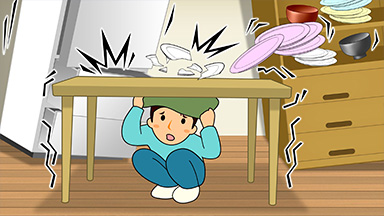
\includegraphics[width=0.5\linewidth]{figures/2017_earthquake1.jpg}		
		\end{center}
		\p{\f{地震}{じしん}が}\p{\f{起}{お}こったら、}\p{テーブルの}\p{\f{下}{した}などに}\p{\f{入}{はい}って、}\p{\f{揺}{ゆ}れが}\p{\f{止}{と}まるまで}\p{\f{待}{ま}ちましょう。}\p{\f{上}{うえ}から}\p{\f{物}{もの}が}\p{\f{落}{お}ちて}\p{きたり、}\p{\f{本棚}{ほんだな}などの}\p{\f{家具}{かぐ}が}\p{\f{倒}{たお}れたり}\p{して}\p{\f{危険}{きけん}だからです。}\p{ストーブや}\p{ガスの}\p{\f{火}{ひ}は、}\p{\f{揺}{ゆ}れが}\p{\f{止}{と}まってから}\p{\f{消}{け}して}\p{ください。}\p{\f{揺}{ゆ}れて}\p{いる}\p{ときに}\p{\f{火}{ひ}を}\p{\f{消}{け}そうと}\p{すると、}\p{やけどを}\p{する}\p{ことが}\p{あります。}
		
		\section{外に逃げるとき}
		\begin{center}
			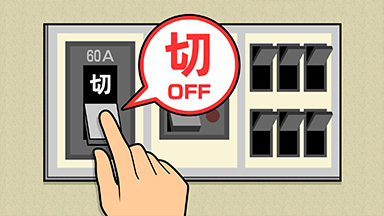
\includegraphics[width=0.5\linewidth]{figures/2017_earthquake2.jpg}		
		\end{center}
		\p{ブレーカーの}\p{スイッチを}\p{「\f{切}{き}る}\p{(\f{off}{おふ})」に}\p{して}\p{\f{電気}{でんき}を}\p{\f{切}{き}ってから、}\p{\f{外}{そと}に}\p{\f{出}{で}て}\p{ください。}\p{\f{大}{おお}きな}\p{\f{地震}{じしん}では}\p{「\f{停電}{ていでん}」に}\p{なって}\p{\f{電気}{でんき}が}\p{\f{止}{と}まる}\p{ことが}\p{あります。}\p{その}\p{あと}\p{\f{電気}{でんき}が}\p{また}\p{\f{流}{なが}れた}\p{ときに、}\p{ストーブなどが}\p{\f{自動}{じどう}で}\p{ついて、}\p{\f{火事}{かじ}に}\p{なる}\p{ことが}\p{あるからです。}
		
		\section{外にいるとき}
		\begin{center}
			
\includegraphics[width=0.5\linewidth]{figures/2017_earthquake3.jpg}		
		\end{center}
		\p{ビルの}\p{\f{近}{ちか}くは、}\p{\f{窓}{まど}}\p{ガラスや}\p{\f{看板}{かんばん}などが}\p{\f{落}{お}ちて}\p{くる}\p{ことが}\p{あります。}\p{かばんなどで}\p{\f{頭}{あたま}を}\p{\f{守}{まも}りながら、}\p{\f{安全}{あんぜん}な}\p{\f{場所}{ばしょ}に}\p{\f{逃}{に}げて}\p{ください。}\p{ブロックの}\p{\f{塀}{へい}や}\p{\f{自動}{じどう}}\p{\f{販売}{はんばい}}\p{\f{機}{き}など}\p{\f{倒}{たお}れやすい}\p{\f{物}{もの}の}\p{\f{近}{ちか}くも}\p{\f{危険}{きけん}です。}\p{\f{山}{やま}や}\p{\f{崖}{がけ}などは}\p{\f{崩}{くず}れて}\p{\f{危険}{きけん}ですから、}\p{\f{遠}{とお}くに}\p{\f{逃}{に}げて}\p{ください。}
		\begin{center}
			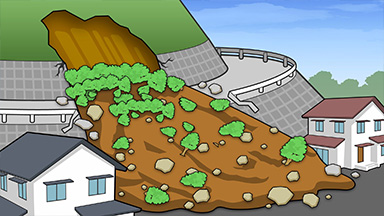
\includegraphics[width=0.5\linewidth]{figures/2017_earthquake4.jpg}		
		\end{center}
		
		\section{車を運転しているとき}
		\p{\f{車}{くるま}を}\p{ゆっくり}\p{\f{道}{みち}の}\p{\f{左側}{ひだりがわ}に}\p{\f{止}{と}めて、}\p{エンジンを}\p{\f{切}{き}ります。}\p{\f{車}{くるま}を}\p{\f{道}{みち}に}\p{\f{置}{お}いて}\p{\f{逃}{に}げる}\p{\f{場合}{ばあい}は、}\p{ドアに}\p{\f{鍵}{かぎ}を}\p{かけないで、}\p{\f{車}{くるま}に}\p{\f{鍵}{かぎ}を}\p{\f{付}{つ}けた}\p{ままに}\p{して}\p{おきましょう。}\p{\f{救急}{きゅうきゅう}\f{車}{しゃ}や}\p{\f{警察}{けいさつ}などの}\p{\f{車}{くるま}が}\p{\f{通}{とお}る}\p{ときに、}\p{\f{動}{うご}かす}\p{ことが}\p{あるからです。}
		
	}
	
	\clearpage
	\titleformat*{\section}{\rmfamily\bfseries}
	\rmfamily
	
	\section*{Vokabular}\noindent
	\begin{multicols}{2}[{\centering\textbf{Bitno}}]
		\dictentry{起こる \strut}{おこる}{\item dogoditi se}{glagol (五)}
		\dictentry{建物 \strut}{たてもの}{\item građevina}{imenica}
		\dictentry{止まる \strut}{とまる}{\item stati}{glagol (五)}
		\dictentry{待つ \strut}{まつ}{\item čekati}{glagol (五)}
		\dictentry{家具 \strut}{かぐ}{\item namještaj}{imenica}
		\dictentry{逃げる \strut}{にげる}{\item pobjeći}{glagol (一)}
		\dictentry{危険 \strut}{きけん}{\item opasnost}{imenica, no-pridjev}
		\dictentry{塀 \strut}{へい}{\item zid}{imenica}
		\dictentry{場合 \strut}{ばあい}{\item situacija, slučaj}{imenica (priložna)}
		\dictentry{通る \strut}{とおる}{\item proći}{glagol (五)}
		\dictentry{動かす \strut}{うごかす}{\item pomaknuti}{glagol (五)}
	\end{multicols}
	\begin{multicols}{2}[{\centering\textbf{Ostalo}}]
		\dictentry{地震 \strut}{じしん}{\item potres}{imenica}
		\dictentry{中 \strut}{なか}{\item unutar, sredina}{imenica}
		\dictentry{下 \strut}{した}{\item ispod, dolje}{imenica}
		\dictentry{入る \strut}{はいる}{\item ući}{glagol (五)}
		\dictentry{揺れ \strut}{ゆれ}{\item trešnja}{imenica}
		\dictentry{上 \strut}{うえ}{\item gore, iznad}{imenica}
		\dictentry{物 \strut}{もの}{\item stvar}{imenica}
		\dictentry{落ちる \strut}{おちる}{\item pasti}{glagol (一)}
		\dictentry{本棚 \strut}{ほんだな}{\item biblioteka}{imenica}
		\dictentry{倒れる \strut}{たおれる}{\item opasti}{glagol (一)}
		\dictentry{火 \strut}{ひ}{\item vatra}{imenica }
		\dictentry{消す \strut}{けす}{\item ugasiti}{glagol (五)}
		\dictentry{外 \strut}{そと}{\item vani}{imenica}
		\dictentry{切る \strut}{きる}{\item rezati, ugasiti}{glagol (五)}
		\dictentry{電気 \strut}{でんき}{\item struja}{imenica}
		\dictentry{出る \strut}{でる}{\item izaći}{glagol (一)}
		\dictentry{大きい \strut}{おおきい}{\item velik}{i-pridjev}
		\dictentry{停電 \strut}{ていでん}{\item nestanak struje}{imenica, suru-glagol (一)}
		\dictentry{流れる \strut}{ながれる}{\item teći}{glagol (一)}
		\dictentry{自動 \strut}{じどう}{\item automatski}{no-pridjev, imenica}
		\dictentry{火事 \strut}{かじ}{\item požar}{imenica}
		\dictentry{近い \strut}{ちかい}{\item blizu}{i-pridjev}
		\dictentry{窓 \strut}{まど}{\item prozor}{imenica}
		\dictentry{看板 \strut}{かんばん}{\item natpis, pano, reklama}{imenica}
		\dictentry{頭 \strut}{あたま}{\item glava}{imenica}
		\dictentry{守る \strut}{まもる}{\item zaštititi}{glagol (五)}
		\dictentry{安全 \strut}{あんぜん}{\item sigurno(-st)}{imenica, na-pridjev}
		\dictentry{場所 \strut}{ばしょ}{\item mjesto}{imenica}
		\dictentry{自動販売機 \strut}{じどうはんばいき}{\item automat}{imenica}
		\dictentry{山 \strut}{やま}{\item planina}{imenica, brojač}
		\dictentry{崖 \strut}{がけ}{\item litica}{imenica}
		\dictentry{崩れる \strut}{くずれる}{\item srušiti se}{glagol (一)}
		\dictentry{遠い \strut}{とおい}{\item dalek}{i-pridjev}
		\dictentry{車 \strut}{くるま}{\item automobil}{imenica}
		\dictentry{運転 \strut}{うんてん}{\item vožnja, voziti}{imenica, no-pridjev, suru glagol (一)}
		\dictentry{道 \strut}{みち}{\item put, cesta}{imenica}
		\dictentry{左側 \strut}{ひだりがわ}{\item lijeva strana}{imenica, no-pridjev}
		\dictentry{置く \strut}{おく}{\item ostaviti}{glagol (五)}
		\dictentry{鍵を付ける \strut}{かぎをかける}{\item zaključati}{izraz}
		\dictentry{救急車 \strut}{きゅうきゅうしゃ}{\item hitna pomoć}{imenica}
		\dictentry{警察 \strut}{けいさつ}{\item policija}{imenica}
	\end{multicols}
	
	\section*{Zadaci}
	\begin{enumerate} 
		\item Sažmite tekst u najviše dvije rečenice.
		\item Razgovarajte o tekstu.
	\end{enumerate}
	
	\section*{Domaća zadaća}
	\begin{enumerate}
		\item Napišite kratku priču ili par rečenica koristeći barem 5 riječi iz teksta. Rečenice ili tekst ne moraju nužno biti vezane uz samu vijest. 
		\item Odgovorite na pitanja:
		\begin{enumerate}[label=(\roman*)]
			\item 地震の時に建物の中にいると何をしなければならないのですか?
			\item 大きな地震の時に何が起こるんですか?
			\item 外にいると何に注意しなければなりませんか?
			\item 何で車に鍵を付けたままにしておくことをしますか?
		\end{enumerate}
		
		\item Nadopunite sljedeće rečenice riječima iz vokabulara:
		\begin{enumerate}[label=(\roman*)]
			\item 危険なものが起こると、すぐに助けを求めてください。
			\item 古い建物の中に家具を見つけたら自分の家に持って帰ることはだめです。
			\item 救急車が止まるまでけが人のそばから離れてわいけません。
			\item 花子ちゃんはライオンから逃げている夢をしたから今は武くんの家の前で彼に夢のことを話したいから待っている。
			\item 鈴木さんは塀を動かそうとしている。
			\item 弾がヘルメットを通った場合に武くんは死ぬだろう。
		\end{enumerate}
	\end{enumerate}
\end{document}